\documentclass[fr]{../../../eplsummary}

\usepackage{../../../eplmath}
\usepackage{multirow}
\usepackage{float}
\usepackage{tikz}
\usepackage{tabularx}
\usepackage[french, ruled, vlined]{algorithm2e}
\usepackage{csquotes}

\usetikzlibrary{matrix}

\SetKwComment{Comment}{$\triangleright$\ }{}
\SetKw{KwDownTo}{down to}

\graphicspath{{img/}}

\newcommand{\Cmn}{\C^{m \times n}}
\newcommand{\Cmm}{\C^{m \times m}}
\newcommand{\Rmn}{\R^{m \times n}}
\newcommand{\Rmm}{\R^{m \times m}}
\newcommand{\Cn}{\C^{n}}
\newcommand{\Cm}{\C^{m}}
\newcommand{\Rm}{\R^{m}}
\newcommand{\frob}[1]{\norm{#1}_{\textnormal{F}}}
\newcommand{\eps}{\varepsilon_{\textnormal{machine}}}
\newcommand{\fl}{\textnormal{fl}}
\newcommand{\ft}{\tilde{f}}
\newcommand{\nnz}{\textnormal{nnz}}
\newcommand{\sA}{\textnormal{sA}}
\newcommand{\iA}{\textnormal{iA}}
\newcommand{\jA}{\textnormal{jA}}

\DeclareMathOperator{\nullspace}{null}
\DeclareMathOperator{\Image}{Im}
\DeclareMathOperator{\range}{range}
\DeclareMathOperator{\rank}{rank}
\DeclarePairedDelimiterX{\inp}[2]{\langle}{\rangle}{#1, #2}
\DeclareMathOperator{\tr}{tr}
\DeclareMathOperator{\sign}{sign}

\hypertitle[']{Analyse numérique}{5}{INMA}{1170}
{Gilles Peiffer}
{François Henrotte et Jean-François Remacle}

% TODO annexe Gmsh (CM2)?
% TODO check for reorganisation?
% TODO explain the last part of CM3 better, cf. slides
% TODO add proof for low-rank approx proofs CM4
% TODO add reference to Higham?
% TODO appendix with example of why classical GS is unstable
% TODO outer product formulation of LU factorization

\section{Fondements}
Dans ce chapitre, nous allons étudier
les bases de l'algèbre linéaire\footnote{\textit{Pun intended\dots}}.
L'algèbre linéaire est l'étude de l'équation
\[
Ax = b\,.
\]
Il y a quatre façons de voir cette équation:
\begin{enumerate}
	\item Comme un \emph{produit matrice-vecteur}, où
	\[
	A \in \Cmn\,, \quad x \in \Cn\,, \quad b \in \Cn\,.
	\]
	\item Comme une \emph{expression tensorielle}:
	\[
	b_i = \sum_{j=1}^{n} a_{ij}x_i\,,
	\]
	où $a_{ij}$ est l'entrée
	à la $i$\ieme{} ligne
	et la $j$\ieme{} colonne de $A$.
	\item Comme disant que
	\emph{$b$ est dans le \textbf{column space} de $A$}\footnote{Espace vectoriel sous-tendu par les colonnes de $A$.},
	et est donc une combinaison linéaire des colonnes de $A$.
	\[
	b = Ax = \sum_{j=1}^{n} x_j a_j\,,
	\]
	où $a_j$ est la $j$\ieme{} colonne de $A$.
	\item Comme une \emph{application linéaire} de $\Cn$ dans $\Cm$:
	\begin{align*}
	A \colon \Cn &\to \Cm\,,\\
	x &\mapsto Ax\,.
	\end{align*}
	On a donc les propriétés suivantes:
	\[
	\begin{array}{rcl@{\quad}l}
		A(x+y) & = & A(x) + A(y)\,, & \quad \forall x,y \in \Cn\,,\\
		A(\alpha x) & = & \alpha A(x)\,, & \quad \forall x \in \Cn\,,
		\quad \alpha \in \C\,.
	\end{array}
	\]
\end{enumerate}

\subsection{Produit matrice-matrice}
Le produit matrice-matrice
\[
B = AC\,, \quad B \in \C^{\ell \times n}\,,\quad A \in \C^{\ell \times m}\,,\quad C \in \Cmn
\]
est une généralisation du produit matrice-vecteur vu précédemment.
On peut également l'écrire
\begin{align*}
	b_{ij} &= \sum_{k=1}^{m} a_{ik}c_{kj}\,.
\end{align*}
Chaque colonne de $B$ est une combinaison linéaire
des colonnes de $A$.

\subsection{Définitions}
\begin{mydef}[Column space]
	Le \emph{column space} d'une matrice $A \in \Cmn$,
	également noté $\range(A)$ est défini comme
	\[
	\range(A) = \mathrm{span}\{a_1, a_2, a_3, \dots, a_n\}\,.
	\]
\end{mydef}
\bigbreak
\begin{mydef}[Kernel]
	Le \emph{kernel} (\emph{noyau}, encore appelé \emph{null space}) d'une matrice $A \in \Cmn$
	est défini comme
	\[
	\nullspace(A) = \set{x \in \Cn \suchthat Ax = 0}\,.
	\]
	Les composantes de chaque vecteur de $\nullspace(A)$
	sont les coefficients d'une combinaison linéaire nulle
	des colonnes de $A$.
	\[
	Ax = 0 \iff \sum_{j=1}^{n} x_j a_j = 0\,.
	\]
\end{mydef}
\bigbreak
\begin{mydef}[Rang]
	Le \emph{rang} d'une matrice $A \in \Cmn$
	est défini comme la dimension de $\range(A)$:
	\[
	\rank(A) = \dim(\range(A))\,.
	\]
	Les espaces vectoriels sous-tendus
	par les lignes et les colonnes d'une matrice (carrée ou rectangulaire)
	ont toujours la même dimension.
	On appelle rang de la matrice $A$ cette dimension.
	On a donc nécessairement
	\[
	\rank(A) \le \min(m,n)\,.
	\]

	On dit qu'une matrice est \emph{de plein rang} lorsque
	\[
	\rank(A) = \min(m,n)\,.
	\]
	Une matrice est de plein rang si et seulement si
	jamais deux vecteurs différents de son domaine n'ont la même image.
	Cela implique que l'application
	\[
	A \colon \Cn \to \range(A) \subseteq \Cm
	\]
	est bijective\footnote{La démonstration est en page 7 du livre.}.
	% TODO add bib reference, maybe put this in an appendix?

	Il n'y a qu'une seule matrice \emph{de rang zéro} par dimension:
	la matrice nulle.

	Pour ce qui en est des matrices \emph{de rang un},
	prenons les vecteurs suivants:
	\begin{align*}
		u &\in \C^{m \times 1}\,,\\
		v &\in \C^{1 \times n}\,.
	\end{align*}
	Leur produit s'écrit
	\[
	\big(uv\big)_{ij} = u_i v_j\,.
	\]
	Cette matrice $\big(uv\big)_{ij}$ est de rang un,
	car toutes ses colonnes sont multiples de $u$.
\end{mydef}
\bigbreak
\begin{mydef}[Matrice inversible]
	Une matrice carrée $A \in \Cmm$ est \emph{inversible}
	si elle satisfait les propositions ci-dessous.
	Toutes les propositions suivantes sont équivalentes:
	\begin{enumerate}[label=(\alph*)]
		\item $A$ est inversible;
		\item $\rank(A) = m$ ($A$ est de plein rang);
		\item $\range(A) = \Cm$;
		\item $\nullspace(A) = \{0\}$ (et \emph{non pas} $\emptyset$);
		\item $0$ n'est pas une valeur propre de $A$;
		\item $0$ n'est pas une valeur singulière de $A$;
		\item $\det(A) \ne 0$.
	\end{enumerate}
\end{mydef}
\bigbreak
\begin{mydef}[Matrice adjointe]
	Si $A \in \Cmn$, la \emph{matrice adjointe} de $A$,
	notée\footnote{Une autre notation possible est $A^{\dag}$.} $A^*$,
	est la matrice obtenue:
	\begin{itemize}
		\item en prenant le complexe conjugué de chaque coefficient;
		\item en permutant lignes et colonnes.
	\end{itemize}
	Remarquons que si $A$ est réelle, $A^* = A^T$.
\end{mydef}
\subsection{Produit scalaire}
Un \emph{produit scalaire} (ou \emph{produit intérieur})
est une opération bilinéaire
\[
\inp{\cdot}{\cdot} \colon \Cm \times \Cm \to \C
\]
telle que
\[
x^* y = \sum_{i=1}^{m} \widebar{x}_i y_i\,,
\]
où $\widebar{x}_i$ est l'entrée $i$ du complexe conjugué de $x$.

Reprenons nos vecteurs $u \in \C^{1 \times m}$
et $v \in \C^{m \times 1}$.
On a que
\[
uv = \sum_{i=1}^{m} u_i v_i\,.
\]
Comme l'opération est bilinéaire,
on a
\[
\renewcommand{\arraystretch}{1.5}
\begin{array}{rcl@{\quad}l}
	\big(x_1 + x_2\big)^* y & = & x_1^* y + x_2^* y\,, & \forall x_1, x_2, y \in \Cm\,,\\
	x^* \big(y_1 + y_2\big) & = & x^* y_1 + x^* y_2\,, & \forall x, y_1, y_2 \in \Cm\,,\\
	\big(ax\big)^* by & = & \widebar{a}b x^* y\,, & \forall a,b \in \C\,, \quad \forall x,y \in \Cm\,.
\end{array}
\]
\subsubsection{Longueur d'un vecteur}
Avec ce produit scalaire,
il est possible de définir la longueur d'un vecteur:
\[
\norm{x} = \sqrt{x^* x}\,, \quad \textnormal{si } x\in \R^{m}\,.
\]

\subsubsection{Angle entre deux vecteurs}
Le produit scalaire permet aussi
de définir l'angle entre deux vecteurs:
\[
\cos \alpha = \frac{x^* y}{\norm{x}\norm{y}}\,.
\]
\subsubsection{Orthogonalité}
Grâce au produit scalaire,
on peut définir le concept d'orthogonalité
\begin{itemize}
	\item de deux vecteurs:
	\[
	x^* y = 0 \iff y^* x = 0\,,
	\]
	\item d'un ensemble $\mathcal{S}$ de vecteurs:
	\[
	x^* y = 0\,, \quad \forall x,y \in \mathcal{S} \suchthat x \ne y \implies \textnormal{ils sont linéairement indépendants,}
	\]
	\item de deux ensembles $\mathcal{S}$ et $\mathcal{S}'$
	de vecteurs non nuls:
	\[
	x^* y = 0\,,\quad \forall x \in \mathcal{S}\,,\quad \forall y \in \mathcal{S}'\,.
	\]
\end{itemize}
\subsubsection{Décomposition orthogonale}
Soit un ensemble $\mathcal{Q} = \{q_1,q_2,\dots,q_n\}$ de vecteurs orthonormés
formant une base orthonormée
pour un sous-espace de dimension $n \le m$ de $\Cm$.
On a alors\footnote{Où $\delta_{ij}$ est le \emph{symbole de Kronecker}.}
\[
q_i^* q_j = \delta_{ij}\,,\quad i,j = 1,\dots,n\,.
\]
Soit $v \in \Cm$.
On a la décomposition orthogonale
\begin{align*}
v &= r + \sum_{i=1}^{n} q_i^* v q_i\\
&= r + \sum_{i=1}^{n} q_i q_i^* v\,,
\end{align*}
avec $q_i^* r = 0$,
c'est-à-dire $r \perp \mathcal{Q}$.
\subsubsection{Matrice unitaire}
Une matrice unitaire est une matrice carrée vérifiant
\[
Q^* = Q^{-1} \iff Q^* Q = I\,,
\]
qui s'écrit également
\[
q_1^* q_2 = \delta_{ij}\,,
\]
en termes des colonnes de $Q$.
Les colonnes d'une matrice unitaire de $\Cmm$
forment une base orthonormée pour $\Cm$.
\subsubsection{Isométrie}
Une matrice unitaire laisse le produit scalaire invariant:
\[
\big(Qx\big)^* Qy = x^* y\,.
\]
Les longueurs des vecteurs et les angles qu'ils forment
sont donc également invariants\footnote{En mécanique des solides déformables,
cela donne lieu aux rotations et aux réflexions
selon que $\det(Q)$ soit $1$ ou $-1$ respectivement.}.
\subsection{Norme vectorielle}
Une norme vectorielle est une fonction
\[
\norm{\cdot} \colon \Cn \to \R
\]
satisfaisant les trois hypothèses suivantes:
\begin{itemize}
	\item \emph{séparation}: $\norm{x} \ge 0$
	avec l'égalité si et seulement si $x = 0$;
	\item \emph{inégalité triangulaire}: $\norm{x+y} \le \norm{x} + \norm{y}$;
	\item \emph{homogénéité absolue}: $\norm{ax} = \abs{a}\norm{x}\,,\quad \forall a \in \C$.
\end{itemize}

\begin{myrem}
	\emph{Le produit scalaire n'est donc pas une norme},
	car il ne satisfait pas la deuxième hypothèse.
	Cependant, sa racine carrée l'est.
\end{myrem}

Il existe beaucoup de normes différentes,
comme par exemple les $p$-normes (ou $\ell^p$-normes):
\begin{itemize}
	\item la norme $\ell^1$ définie par
	\[
	\norm{x}_1 \coloneqq \sum_i \abs{x_i}\,;
	\]
	\item la norme $\ell^2$ définie par
	\[
	\norm{x}_2 \coloneqq \sqrt{\sum_i x_i^2}\,;
	\]
	\item la norme $\ell^p$ définie par
	\[
	\norm{x}_p \coloneqq \left(\sum_i \abs{x_i}^p\right)^{1/p}\,;
	\]
	\item la norme $\ell^{\infty}$ définie par
	\[
	\norm{x}_\infty \coloneqq \max_i \abs{x_i}\,.
	\]
\end{itemize}
On peut donner une représentation graphique de ces normes vectorielles.
On définit pour cela les \emph{boules unitaires} (\emph{unit balls}):
\[
B_p^m = \set[\big]{x \in \Cm \suchthat \norm{x}_p \le 1}\,.
\]
\begin{figure}[H]
	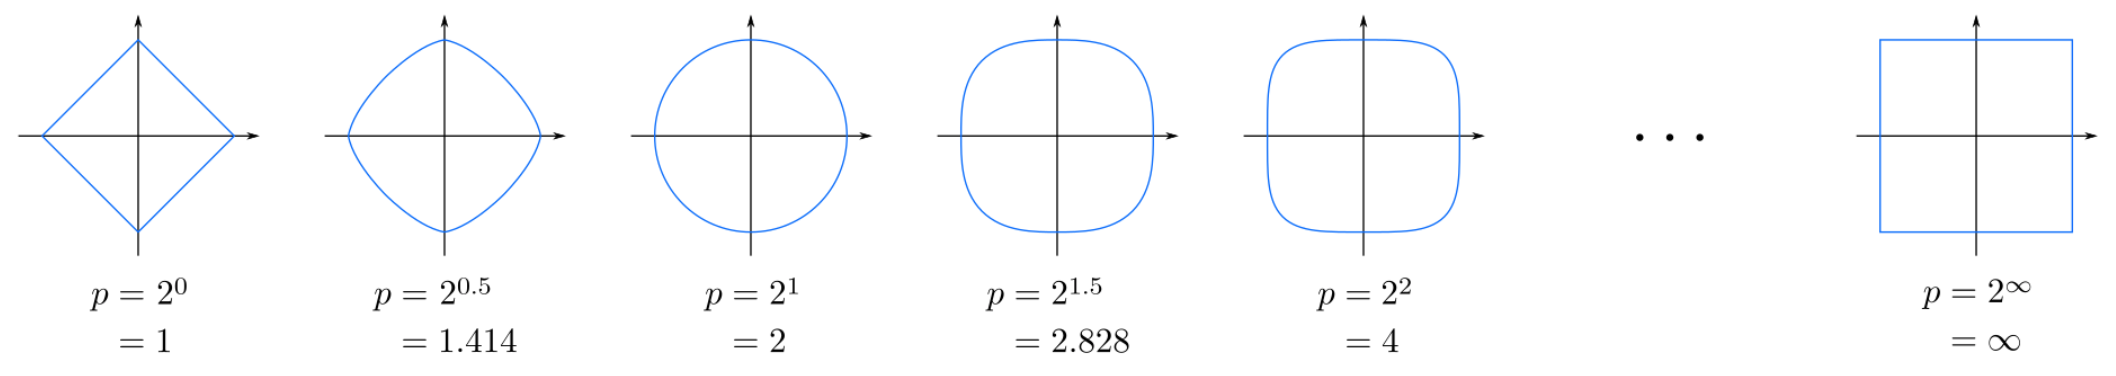
\includegraphics[width=\textwidth]{unit_balls.png}
	\caption{Une visualisation des boules $B_p^1$ pour $p \in \intervalco{1}{+\infty}$.}
	\label{fig:unit_balls}
	% TODO bib ref (wikipedia; unit ball)
\end{figure}
Comme on le voit sur la figure,
\[
B_p^m \subsetneq B_q^m\,,\quad \forall p < q\,.
\]
\subsection{Norme matricielle}
La norme matricielle induite par une norme vectorielle
est une norme pour les matrices
regardées comme des opérateurs sur les vecteurs.
Soit $A \in \Cmn$ un opérateur $A \colon \Cn \to \Cm$
et $\norm{\cdot}_{(m)}$ et $\norm{\cdot}_{(n)}$ deux normes vectorielles
respectivement sur $\Cm$ et $\Cn$.
On définit la norme matricielle $\norm{\cdot}_{(m,n)}$
induite par ces normes vectorielles par
\[
\norm{A}_{(m,n)} \coloneqq \sup_{x \in \Cn \setminus \{0\}} \frac{\norm{Ax}_{(m)}}{\norm{x}_{(n)}}\,.
\]
Comme toute norme doit satisfaire l'hypothèse d'homogénéité absolue,
et que $A$ est linéaire,
on voit que la norme de $x$ n'intervient pas dans la norme matricielle.
On peut également définir cette norme sans division:
\[
\norm{A}_{(m,n)} \coloneqq \sup_{x \in B_p^m} \norm{Ax}_{(m)}\,.
\]
On a l'égalité pratique suivante:
\[
\norm{A}_{(m, n)} \ge \frac{\norm{Ax}_{(m)}}{\norm{x}_{n}}\,.
\]

\subsubsection{$\norm{A}_1$}
\label{sec:1-norm}
% TODO cite example 3.3 in book
Soit la 1-norme matricielle $\norm{\cdot}_1$
induite par les normes vectorielles
$\norm{\cdot}_{(m)} = 1$ et $\norm{\cdot}_{(n)} = 1$.
Soit $A \in \Cmn$.
On prend $x \in B_{1}^{n}$,
et on écrit (où $a_j$ est la $j$\ieme{} colonne de $A$)
\begin{align*}
\norm{Ax}_1 &= \norm{\sum_{j=1}^{n} x_j a_j}_1 \\
&\le \sum_{j=1}^{n} \abs{x_j} \norm{a_j}_1 \\
&\le \max_{1 \le j \le n} \norm{a_j}_1\,.
\end{align*}
On en déduit que
\[
\norm{A}_1 \le \max_{1 \le j \le n} \norm{a_j}_1\,.
\]
Si on choisit $x = e_j$,
où $j$ maximise $\norm{a_j}_1$,
on atteint cette borne,
et donc la norme matricielle est le ``\emph{maximum column sum}'':
\[
\norm{A}_1 = \max_{1 \le j \le n} \norm{a_j}_1\,.
\]

\subsubsection{$\norm{A}_{\infty}$}
% TODO cite example 3.4 in book
Soit $A \in \Cmn$.
On prend $x \in B_{\infty}^{n} \implies \abs{x_j} \le 1 \quad \forall j$.
\begin{align*}
	\norm{Ax}_{\infty} &= \norm{\sum_{j=1}^{n} x_j a_j}_{\infty} \\
	&= \sum_{j=1}^{n} \norm{x_j a_j}_{\infty} \\
	&\le \sum_{j=1}^{n} \abs{x_j} \norm{a_j}_{\infty} \\
	&= \sum_{j=1}^{n} \abs{x_j} \max_{1 \le i \le m} a_{ij} \\
	&\le \sum_{j=1}^{n} \max_{1 \le i \le m} a_{ij} \\
	&= \max_{1 \le i \le m} \sum_{j=1}^{n} \abs{a_{j}} \\
	&= \max_{1 \le i \le m} \norm{a_i^*}_1\,.
\end{align*}
On applique le même raisonnement qu'à la \sectionref{1-norm}
pour trouver que la borne est serrée et égale au ``\emph{maximum row sum}'':
\[
\norm{A}_{\infty} = \max_{1 \le i \le m} \norm{a_i^*}_1\,.
\]

\subsubsection{Borner $\norm{AB}$}
Soient $\norm{\cdot}_{(\ell)}$,
$\norm{\cdot}_{(m)}$ et $\norm{\cdot}_{(n)}$
des $p$-normes vectorielles pour $\C^{\ell}$, $\Cm$ et $\Cn$ respectivement.
Soient $A \in \C^{\ell \times m}$ et $B \in \Cmn$.
On sait que
\begin{align*}
\norm{ABx}_{(\ell)} &\le \norm{A}_{(\ell, m)} \norm{Bx}_{(m)}\\
&\le \norm{A}_{(\ell, m)} \norm{B}_{(m, n)} \norm{x}_{(n)}\,.
\end{align*}
On trouve alors
\[
\norm{AB}_{(\ell, n)} \le \norm{A}_{(\ell, m)} \norm{B}_{(m, n)}\,.
\]
Notons qu'en général, cette inégalité n'est pas serrée.

\subsection{Inégalités de Cauchy-Schwarz et de Hölder}
Calculer les $p$-normes matricielles avec $p \ne 1, \infty$ est compliqué,
et afin de résoudre ce problème,
on note que les produits intérieurs peuvent être bornés
en utilisant des $p$-normes.
Soient $p$ et $q$ tels que
\[
\frac{1}{p} + \frac{1}{q} = 1\,, \quad 1 \le p, q \le \infty\,.
\]
L'\emph{inégalité de Hölder} dit alors que,
pour tout vecteurs $x$ et $y$,
\[
\abs{x^* y} \le \norm{x}_p \norm{y}_q\,.
\]
Dans le cas particulier $p = q = 2$,
on a l'\emph{inégalité de Cauchy-Schwarz}:
\[
\abs{x^* y} \le \norm{x}_2 \norm{y}_2\,.
\]
Ces deux bornes sont serrées.

\begin{myrem}
	Deux remarques sont à faire ici:
	\begin{itemize}
		\item Il ne faut pas confondre cette inégalité
		avec l'inégalité triangulaire qui implique une somme.
		\item Cette inégalité n'est valable que pour certaines normes.
	\end{itemize}
\end{myrem}

\subsection{Norme de Frobenius}
La norme de Frobenius\footnote{Également appelée norme de Hilbert-Schmidt.} d'une matrice
n'est pas induite par une norme vectorielle.
Pour être une norme matricielle,
il suffit que la norme vérifie les trois propriétés des normes vectorielles,
appliquées dans l'espace vectoriel des matrices, de dimension $mn$.
La norme de Frobenius est définie comme
\begin{align*}
\frob{A} &= \left(\sum_{i=1}^{m} \sum_{j=1}^{n} \abs{a_{ij}^2}\right)^{1/2} \\
&= \left(\sum_{j=1}^{n} \norm{a_{j}}_2 \right)^{1/2} \\
&= \sqrt{\tr(A^* A)}\,.
\end{align*}

\begin{mytheo}[Invariance sous multiplication unitaire]
La norme de Frobenius et la $2$-norme matricielle sont invariantes
sous multiplication par une matrice unitaire,
c'est-à-dire que pour tout $A \in \Cmn$, et $Q \in \Cmm$ unitaire,
on a
\[
\norm{QA}_2 = \norm{A}_2 \quad \textnormal{et} \quad \frob{QA} = \frob{A}\,.
\]
\end{mytheo}

La norme de Frobenius peut être utilisée pour borner un produit de matrices.
Posons $C = AB$ avec $C \in \C^{n \times m}$
dont les entrées sont les $c_{ik} = a_i^* b_j$.
Par l'inégalité de Cauchy-Schwarz,
on a alors $\abs{c_{ij}} \le \norm{a_i}_2 \norm{b_j}_2$.
En mettant au carré des deux cotés et en sommant, on trouve
\begin{align*}
	\frob{C}^2 = \frob{AB}^2 &= \sum_{i=1}^{n} \sum_{j=1}^{m} \abs{c_{ij}^2} \\
	&\le \sum_{i=1}^{n} \sum_{j=1}^{m} \left(\norm{a_i}_2 \norm{b_j}_2 \right)^2 \\
	&= \sum_{i=1}^{n} \left( \norm{a_i}_2 \right)^2 \sum_{j=1}^{m} \left( \norm{b_j}_2 \right)^2 \\
	&= \frob{A}^2 \frob{B}^2\,.
\end{align*}

\section{Factorisation QR}
\subsection{Projecteurs}
\begin{mydef}[Projecteur]
	Un \emph{projecteur} est une matrice carrée $P$
	qui satisfait l'équation
	\[
	P^2 = P\,.
	\]
	Une telle matrice est également appelée \emph{idempotente}.
	On distingue les projecteurs orthogonaux et non orthogonaux.
	Un projecteur n'a que deux valeurs propres potentielles: $0$ et $1$.
	Si le projecteur $P$ est symétrique, alors
	\[
	\Image P \perp \ker P\,.
	\]
\end{mydef}

On définit un projecteur ``fondamental''\footnote{Nom donné par le professeur.}
tel que
\begin{align*}
P &= \frac{vv^*}{\norm{v}_2^2} = \frac{vv^*}{v^* v} \\
\implies P^2 &= \frac{(v v^*) (v v^*)}{\norm{v}_2^4} = \frac{v v^* \norm{v}_2^2}{\norm{v}_2^4} = \frac{vv^*}{\norm{v}_2^2} = P\,.
\end{align*}

On définit également un projecteur complémentaire à $P$, $I - P$.
\[
(I - P)^2 = I^2 - 2P + P^2 = I - P\,.
\]

\subsection{Réflecteurs de Householder}
Définissons une application linéaire $F$
et appelons-là \emph{réflecteur de Householder}.
Prenons un point $x$ et un hyperplan $H$ défini comme
l'ensemble des points orthogonaux
à un vecteur non nul fixe $v = \norm{x}e_1 - x$.

Lorsque le réflecteur est appliqué,
tout point d'un coté de $H$ est envoyé sur son image de l'autre coté.
En particulier, $x$ est envoyé sur $\norm{x} e_1$.
La formule de cette réflection se dérive de la façon suivante:
on voit facilement que la projection orthogonale de $y \in \Cm$ sur $H$
est donnée par
\[
Py = \left( I - \frac{v v^*}{v^* v} \right) y = y - v \left( \frac{v^* y}{v^* v} \right)\,.
\]
Afin de terminer la réflection, on ne peut pas encore s'arrêter là;
il faut se déplacer dans cette direction une fois de plus.
La réflection $Fy$ devrait donc être
\[
Fy = \left( I - 2 \frac{v v^*}{v^* v} \right) y = y - 2v \left( \frac{v^* y}{v^* v} \right)\,.
\]
On déduit alors que la matrice $F$ est
\[
F = I - 2 \frac{v v^*}{v^* v}\,.
\]
On vérifie facilement que cette matrice est unitaire
car $F^2 = I$ et donc $F = F^*$.
Comme la matrice est inversible, elle est de plein rang.

\subsection{Factorisation \textsc{qr}}
Soit une matrice $A \in \Cmn$.
On suppose que
\[
A = QR\,, \quad Q \in \Cmm \textnormal{ unitaire,} \quad R \in \Cmn \textnormal{ triangulaire supérieure.}
\]
On voit direct que cette façon d'encoder $A$ n'est pas optimale:
$A$ a $mn$ éléments, alors que $Q$ et $R$ ensemble en ont $m(m+n)$.
Cependant, on sait que $R$ est triangulaire supérieure
et que $Q$ est unitaire
(et on connaît donc les valeurs des ses éléments diagonaux).
Schématiquement, on a donc quelque chose de la forme suivante
(ici pour $(m, n) = (5, 3)$):
\[
\begin{tikzpicture}[baseline=(current bounding box.center)]
\matrix[matrix of math nodes,execute at empty cell={\node[black!20]{0};},%Node color and text "0"
        every left delimiter/.style={xshift=1ex},%tighter delimiter spacing
        every right delimiter/.style={xshift=-1ex},
                left delimiter={(},right delimiter={)}
                ] {
a_{11} & a_{12} & a_{13} \\
a_{21} & a_{22} & a_{23} \\
a_{31} & a_{32} & a_{33} \\
a_{41} & a_{42} & a_{43} \\
a_{51} & a_{52} & a_{53} \\
};
\end{tikzpicture}
=
\begin{tikzpicture}[baseline=(current bounding box.center)]
\matrix[matrix of math nodes,execute at empty cell={\node[black!20]{\times};},%Node color and text "0"
        every left delimiter/.style={xshift=1ex},%tighter delimiter spacing
        every right delimiter/.style={xshift=-1ex},
                left delimiter={(},right delimiter={)}
                ] {
       &        &        &        &        \\
q_{21} &        &        &        &        \\
q_{31} & q_{32} &        &        &        \\
q_{41} & q_{42} & q_{43} &        &        \\
q_{51} & q_{52} & q_{53} &        &        \\
};
\end{tikzpicture}
\begin{tikzpicture}[baseline=(current bounding box.center)]
\matrix[matrix of math nodes,execute at empty cell={\node[black!20]{0};},%Node color and text "0"
        every left delimiter/.style={xshift=1ex},%tighter delimiter spacing
        every right delimiter/.style={xshift=-1ex},
                left delimiter={(},right delimiter={)}
                ] {
r_{11} & r_{12} & r_{13} \\
       & r_{22} & r_{23} \\
       &        & r_{33} \\
       &        &        \\
       &        &        \\
};
\end{tikzpicture}
\]
On a donc bien $mn$ entrées utiles dans $Q$ et $R$ combinés.

On obtient l'algorithme de factorisation suivant
(où on définit $\sign(x) = 1$ si $x = 0$):

\begin{algorithm}[H]
\DontPrintSemicolon
\KwData{Une matrice $A \in \Cmn$.}
\KwResult{La matrice triangulaire supérieure $R \in \Cmn$
dans la décomposition \textsc{qr} de $A$.}
\Begin{
	\For{$k \gets 1$ \KwTo $n$}{
	$x \gets A_{k {:} m, k}$\;
	$v_k \gets \sign(x_1)\norm{x}_2 e_1 + x$\;
	$v_k \gets v_k / \norm{v_k}_2$\;
	$A_{k {:} m, k {:} n} \gets A_{k {:} m, k {:} n} - 2 v_k(v_k^* A_{k {:} m, k {:} n})$\;
	}
	\Return $A$\;
}
\caption{Factorisation \textsc{qr} de Householder\label{algo:qr_householder}}
\end{algorithm}

Cet algorithme a une complexité qui se calcule relativement facilement:
soit $w(m, n)$ la fonction qui compte le nombre d'opérations
en fonction de la taille d'entrée.
\begin{align*}
w(m, n) &\sim \sum_{k=1}^{n} \big( 4 \left( n-k+1 \right)\left( m-k+1 \right) \big) \\
&\sim \frac{2}{3}n(n+1)(3m-n+1) \\
&\sim 2mn^2+2mn-\frac{2n^3}{3}+\frac{2n}{3} \\
&\sim 2mn^2-\frac{2n^3}{3} \\
\overset{m=n}{\implies} w(n) &\sim \frac{4}{3}n^3\,.
\end{align*}

Ensuite, après avoir trouvé cette matrice $R$,
on utilise les différents vecteurs $v_k$
afin d'assembler le produit $Q^* b$ sans calculer $Q$ explicitement.

\begin{algorithm}[H]
\DontPrintSemicolon
\KwData{$b$ et les vecteurs $v_k$ servant à assembler $Q$.}
\KwResult{Le produit $Q^* b$.}
\Begin{
	\For{$k \gets 1$ \KwTo $n$}{
	$b_{k {:} m} \gets b_{k {:} m} - 2 v_k(v_k^* b_{k {:} m})$\;
	}
	\Return $b$\;
}
\caption{Calcul implicite d'un produit $Q^* b$\label{algo:qr_q*b}}
\end{algorithm}

Cet algorithme est de complexité $\bigoh(mn)$.

Finalement, on trouve alors $x$ par substitution arrière
(car $R$ est triangulaire supérieure).

\begin{algorithm}[H]
\DontPrintSemicolon
\KwData{Le vecteur $b$
et la matrice triangulaire supérieure $R$.}
\KwResult{Le vecteur $x$ dans $Rx = b$.}
\Begin{
	\For{$k \gets m$ \KwDownTo $1$}{
	$x_{j} \gets \left.\left(b_{j} - \sum\limits_{k = j+1}^{m} x_k r_{jk} \right)\right/ r_{jj}$\;
	}
	\Return $x$\;
}
\caption{Substitution arrière\label{algo:back_substitution}}
\end{algorithm}

Cet algorithme a une complexité $b(m)$ égale à
\begin{align*}
b(m) &\sim \sum_{j=1}^{m} \big(2(m - j) + 1 \big) \\
&\sim 2 \sum_{k=0}^{m-1} k + m \\
&\sim m (m - 1) + m \\
&\sim m^2\,.
\end{align*}

Cependant, ces trois algorithmes se font séquentiellement,
et la complexité totale de résolution d'un système linéaire
avec une factorisation \textsc{qr} est donc
\[
t(n) \sim \frac{4}{3} n^3\,.
\]
\section{Décomposition en valeurs singulières}
La décomposition en valeurs singulières
(\emph{singular value decomposition} en anglais)
est la généralisation pour les matrices quelconques
de la décomposition en éléments propres.

\begin{mytheo}[Theorème spectral]
	Toute matrice carrée $A$ normale
	(c'est-à-dire telle que $AA^* = A^*A$)
	peut être diagonalisée par une base orthonormée de vecteurs propres.
\end{mytheo}
\begin{mydef}[$n$-sphère]
Nous définissons la $n$-sphère comme
\[
S^n = \{x \in \R^{n+1} \colon \norm{x} = r\}\,.
\]
On peut alors définir la $n$-sphère unité comme le cas particulier $r = 1$.
Nous prenons en général comme norme la $2$-norme vectorielle.
\end{mydef}

La \textsc{svd} est motivée par l'observation géométrique suivante:
\begin{center}
	L'image de la $n$-sphère unité par une matrice $m \times n$ quelconque
	est une hyperellipse.
\end{center}
Bien que la décomposition en valeurs singulières
ne soit pas unique aux matrices réelles,
nous considérons ici le cas $A \in \Rmn$.
\begin{mydef}[Hyperellipse]
	Une \emph{hyperellipse} est
	la généralisation à $m$ dimensions d'une ellipse.
	On peut définir une hyperellipse dans $\Rm$ comme la surface obtenue
	en étirant la $n$-sphère unité dans $\Rm$
	par des facteurs multiplicatifs
	$\sigma_1, \ldots, \sigma_m$ (potentiellement nuls)
	dans des directions orthogonales $u_1, \ldots, u_m \in \Rm$.
\end{mydef}
On peut dire sans perte de généralité que $\norm{u_i}_2 = 1$.
Les vecteurs $\{\sigma_i u_i\}$
sont les demi-axes principaux de l'hyperellipse,
avec pour longueurs $\sigma_1, \ldots, \sigma_m$.
Si la matrice $A$ est de rang $r$,
exactement $r$ des longueurs $\sigma_i$ seront non nulles,
et en particulier si $m \ge n$,
au plus $n$ d'entre-elles seront non nulles.

\subsection{\textsc{svd} réduite}
Supposons $\rank(A) = n$ ($A$ de plein rang);
l'image de $S^{n}$ par $A$, $AS^{n}$, est une hyperellipse dans $\Rn$.
On obtient alors trois choses:
\begin{itemize}
	\item $n$ valeurs singulières de $A$
	(conventionnellement ordonnées de façon décroissante)
	$\sigma_1 \ge \sigma_2 \ge \cdots \ge \sigma_n \ge 0$.
	Elles sont stockées sur
	la diagonale principale de la matrice $\hat{\Sigma} \in \Rnn$.
	\item $n$ vecteurs de base orthonormés $\{u_1, \ldots, u_n\} \in \Rm$
	dits de ``sortie'' ou ``à gauche''.
	Ils sont stockés dans une matrice $\hat{U} \in \Rmn$.
	\item $n$ vecteurs de base orthonormés $\{v_1, \ldots, v_n\} \in \Rn$
	dits d'``entrée'' ou ``à droite''.
	Ils sont stockés dans une matrice unitaire $V \in \Rnn$.
\end{itemize}
On écrit alors
\[
A v_j = \sigma_j u_j\,, \quad 1 \le j \le n\,,
\]
ou bien plus de façon plus compacte
\begin{align*}
AV &= \hat{U} \hat{\Sigma}\,.\\
\intertext{Or $V$ est unitaire; on écrit alors}
A &= \hat{U} \hat{\Sigma} V^*\,.
\end{align*}
Cette factorisation s'appelle
la \emph{décomposition en valeurs singulières réduite},
ou bien \emph{reduced singular value decomposition} en anglais.

\subsection{\textsc{svd} complète}
Pour les matrices $A$ qui ne sont pas de rang plein,
la formulation est légèrement différente.
Si l'on définit $U \in \Cmm$ comme la matrice $\hat{U}$
à laquelle on a ajouté $m-n$ colonnes orthonormeés,
on peut résoudre ce problème.
Il faut cependant encore modifier légèrement $\hat{\Sigma}$,
de sorte à obtenir $\Sigma \in \Rmn$ qui n'est autre
que $\hat{\Sigma}$ en dessous de laquelle
nous avons ajouté $m-n$ lignes de zéros.
On écrit alors
\[
A = U \Sigma V^*\,.
\]
On note que la matrice $U$ est unitaire.

Pour revenir sur l'interprétation géométrique,
nous observons que cette décomposition montre bien les différentes étapes:
\begin{itemize}
	\item l'application unitaire $V^*$ préserve la $n$-sphère;
	\item la matrice diagonale $\Sigma$ étire la $n$-sphère
	de sorte à former une hyperellipse alignée avec la base canonique et
	\item l'application unitaire finale $U$
	reflette ou fait tourner l'hyperellipse sans changer sa forme.
\end{itemize}
Ainsi, si nous arrivons à prouver que toute matrice a une \textsc{svd},
nous aurons également prouvé que
l'image de la $n$-sphère unité sous n'importe quelle application linéaire
est une hyperellipse.

\subsection{Existence et unicité}
\begin{mytheo}[Existence et unicité de la décomposition en valeurs singulières]
Toute matrice $A \in \Cmn$ a une décomposition en valeurs singulières.
De plus, les valeurs singulières $\{\sigma_j\}$
sont univoques (\emph{uniquely determined})
et si $A$ est carrée et les $\sigma_j$ sont distincts, alors
les vecteurs $\{u_j\}$ et $\{v_j\}$ sont univoques à une phase près.
\begin{proof}
	Afin de prouver l'existence de la \textsc{svd},
	nous isolons la direction de plus grande action de $A$,
	et procédons ensuite par induction sur la dimension de $A$.

	Supposons $\sigma_1 = \norm{A}_2 = \sup_{S^n} \norm{Ax}_2$.
	Par un argument de compacité,
	il doit y avoir des vecteurs $v_1 \in \Cn$ et $u_1 \in \Cm$
	tels que $\norm{v_1}_2 = \norm{u_1}_2 = 1$ et $A v_1 = \sigma_1 u_1$.
	Considérons une quelconque extension de $v_1$
	à une base orthonormée $\{v_j\}$ de $\Cn$
	et de $u_1$ à une base orthonormée $\{u_j\}$ de $\Cm$,
	et soient $U_1$ et $V_1$ les matrices unitaires
	avec comme colonnes $u_j$ et $v_j$ respectivement.
	On a alors
	\[
	U_1 A V_1 = S =
	\begin{pmatrix}
		\sigma_1 & w^*\\
		0        & B
	\end{pmatrix}\,,
	\]
	où $0$ est un vecteur colonne de dimension $m-1$,
	$w^*$ est un vecteur ligne de dimension $n-1$
	et $B$ est de dimension $(m-1) \times (n-1)$.
	De plus,
	\[
	\norm{\begin{pmatrix}
		\sigma_1 & w^*\\
		0        & B
	\end{pmatrix}\begin{pmatrix}
		\sigma_1 \\
		w
	\end{pmatrix}}_2 \ge \sigma_1^2 + w^* w = (\sigma_1^2 + w^* w)^{1/2}\norm{\begin{pmatrix}
		\sigma_1 \\
		w
	\end{pmatrix}}_2\,,
	\]
	impliquant $\norm{S}_2 \ge (\sigma_1^2 + w^* w)^{1/2}$.
	Comme $U_1$ et $V_1$ sont unitaires,
	on sait que $\norm{S}_2 = \norm{A}_2 = \sigma_1$,
	et on déduit donc que $w = 0$.
	Si $m = 1$ ou $n = 1$, cela termine la preuve.
	Sinon la sous-matrice $B$ décrit l'action de $A$
	sur le sous-espace orthogonal à $v_1$.
	Par l'hypothèse d'induction,
	la \textsc{svd} de $B$ existe et est donnée par $B = U_2 \Sigma_2 V_2^*$.
	On vérifie alors facilement
	(il suffit de démontrer que les termes
	à gauche et à droite de la matrice diagonale sont unitaires) que
	\[
	A = U_1 \begin{pmatrix}
	1 & 0\\
	0 & U_2
	\end{pmatrix}
	\begin{pmatrix}
	\sigma_1 & 0\\
	0        & \Sigma_2
	\end{pmatrix}
	\begin{pmatrix}
	1 & 0\\
	0 & V_2
	\end{pmatrix}^*
	V_1^*
	\]
	est une \textsc{svd} de $A$, ce qui termine la preuve d'existence.

	En ce qui concerne l'unicité,
	la justification géométrique est directe:
	si les longueurs de demi-axe d'une hyperellipse sont distinctes,
	alors les demi-axes eux-mêmes sont déterminés par la géométrie,
	au signe près.
	Algébriquement, on note d'abord que $\sigma_1$
	est univoque.
	Supposons maintenant qu'en plus de $v_1$,
	il y ait un autre vecteur linéairement indépendant $w$
	tel que $\norm{w}_2 = 1$ et $\norm{Aw}_2 = \sigma_1$.
	Définissons un vecteur unitaire $v_2$, orthogonal à $v_1$,
	comme une combinaison linéaire de $v_1$ et $w$,
	\[
	v_2 = \frac{w - \big(v_1^* w\big) v_1}{\norm{w - \big(v_1^* w \big) v_1}_2}\,.
	\]
	Comme $\norm{A}_2 = \sigma_1$, $\norm{Av_2}_2 \le \sigma_1$;
	or cela doit être une égalité,
	car sinon, comme $w = v_1 c + v_2 s$
	pour des constantes $c$ et $s$
	telles que $\abs{c}^2 + \abs{s}^2 = 1$,
	on aurait $\norm{Aw}_2 < \sigma_1$.
	Ce vecteur $v_2$ est un deuxième vecteur singulier à droite de $A$
	correspondant à la valeur singulière $\sigma_1$;
	il va mener à l'apparition d'un vecteur $y$
	(égal aux $n-1$ dernières composantes de $V_1^*v_2$)
	tel que $\norm{y}_2 = 1$ et $\norm{By}_2 = \sigma_1$.
	On conclut que si le vecteur singulier $v_1$ n'est pas unique,
	alors la valeur singulière $\sigma_1$ correspondante n'est pas simple.
	Afin de terminer la preuve d'unicité,
	nous notons comme indiqué ci-dessus
	qu'une fois $\sigma_1, v_1$ et $u_1$ déterminés de façon univoque,
	la reste de la \textsc{svd} est déterminée par l'action de $A$
	sur le sous-espace orthogonal à $v_1$.
	Comme $v_1$ est unique à un signe près,
	cet espace orthogonal est univoque,
	et l'unicité des valeurs et vecteurs singuliers restants
	est assurée par induction.
\end{proof}
\end{mytheo}
\subsection{Interprétation de la \textsc{svd}}
La \textsc{svd} nous permet de dire que
toute matrice est diagonale--à condition d'utiliser les bonnes bases
pour le domaine et l'image.
Tout $b \in \Cm$ peut s'exprimer
dans la base des vecteurs singuliers à gauche de $A$ (colonnes de $U$)
et tout $x \in \Cn$ peut s'exprimer
dans la base des vecteurs singuliers à droite de $A$ (colonnes de $V$).
On écrit alors
\[
b' = U^* b\,, \quad x' = V^* x\,.
\]
On peut alors réécrire
\[
b = Ax \iff U^* b = U^* Ax \iff b' = U^* U \Sigma V^* x \iff b' = \Sigma x'\,.
\]
$A$ se réduit donc en la matrice diagonale $\Sigma$
lorsque l'image est exprimée dans la base formée par les colonnes de $U$
et que le domaine est exprimé dans la base des colonnes de $V$.
\subsection{\textsc{svd} vs décomposition en valeurs propres}
Ce même principe de \emph{diagonalisation}
est également sous-jacent à l'étude des valeurs propres.
Une matrice régulière $A$ peut être exprimée
comme une matrice diagonale de valeurs propres $\Lambda \in \Cmm$,
à condition que le domaine et l'image soient représentés
dans la base des vecteurs propres.

Si les colonnes d'une matrice $X \in \Cmm$
contiennent des vecteurs linéairement indépendants de $A \in \Cmm$,
la décomposition en valeurs propres de $A$ est
\[
A = X \Lambda X^{-1}\,,
\]
Cela implique que si nous définissons pour $b, x \in \Cm$ tels que $b = Ax$,
\[
b' = X^{-1}b\,, \quad x' = X^{-1}x\,,
\]
alors $b'$ et $x'$ satisfont $b' = \Lambda x'$.

La \tabref{SVDvsEVD} reprend quelques différences
entre ces deux factorisations.
\begin{table}[H]
	\centering
	\begin{tabular}{l p{0.35\linewidth} p{0.35\linewidth}}
		\hline
		\\
		\multicolumn{1}{c}{Critère} & \multicolumn{1}{c}{\textsc{svd}} & \multicolumn{1}{c}{\textsc{evd}}\\\\
		\multirow{2}{*}{Bases et orthogonalité} & Deux bases orthonormées ($\{u_j\}$ et $\{v_j\}$) & Une base non orthogonale ($\{X\}$)\\\\
		\multirow{2}{*}{Existence} & Existe pour toute matrice (même rectangulaire) & N'existe pas pour toute matrice (même carrée) \\\\
		\multirow{2}{*}{Applications} & Problèmes sur les formes itérées de $A$ ($A^k$ ou $\mathrm{e}^{tA}$) & Problèmes sur $A$ ou son inverse\\
		\hline
	\end{tabular}
	\caption{Différences entre
	la décomposition en valeurs singulières (\textsc{svd})
	et la décomposition en valeurs propres (\textsc{evd}).}
	\label{tab:SVDvsEVD}
\end{table}
\subsection{Propriétés des matrices par la \textsc{svd}}
\begin{mytheo}
	Le rang de $A$ est $r$, le nombre de valeurs singulières non nulles.
	\begin{proof}
		Le rang d'une matrice diagonale
		est égal au nombre d'entrées non nulles,
		et dans la décomposition $A = U\Sigma V^*$,
		$U$ et $V$ sont de plein rang.
		Dès lors, $\rank(A) = \rank(\Sigma) = r$.
	\end{proof}
\end{mytheo}
\begin{mytheo}
	$\range(A) = \langle u_1, \ldots, u_r \rangle$ et $\nullspace(A) = \langle v_{r+1}, \ldots, v_n$.
	\begin{proof}
		Ceci est une conséquence du fait que
		$\range(\Sigma)
		= \langle e_1, \ldots, \e_r \rangle \subseteq \Cm$ et
		que $\nullspace(\Sigma)
		= \langle e_{r+1}, \ldots, e_n \rangle \subseteq \Cn$.
	\end{proof}
\end{mytheo}
\subsection{Approximation de rang faible}
\begin{mytheo}[Approximation par des matrices de rang un]
	$A$ peut être écrite comme une somme de $r$ matrices de rang un:
	\[
	A = \sum_{j = 1}^{r} \sigma_j u_j v^*_j\,.
	\]
\end{mytheo}
\begin{mytheo}[Optimalité de la somme des $\nu$ premières approximations de rang un]
	Pour tout $\nu$ tel que $0 \le \nu \le r$, nous définissons
	\[
	A_{\nu} = \sum_{j=1}^{\nu} \sigma_j u_j v_j^*\,;
	\]
	si $\nu = p = \min\{m, n\}$, définissons $\sigma_{\nu+1} = 0$.
	On a alors que
	\[
	\norm{A - A_{\nu}}_2 = \inf_{\substack{B \in \Cmn \\ \rank(B) \le \nu}} \norm{A - B}_2 = \sigma_{\nu + 1}\,.
	\]
\end{mytheo}
\section{Orthogonalisation de Gram-Schmidt}
\subsection{Forme classique}
\label{sec:gsclassical}
Nous cherchons à trouver les colonnes $\{q_j\}$
de la matrice $\hat{Q} \in \Cm$
par un procédé d'orthogonalisation successive.
Ce procédé est appelé \emph{orthogonalisation de Gram-Schmidt}.
À l'étape $j$, nous cherchons à trouver
un vecteur unitaire $q_j \in \langle a_1, \ldots, a_j \rangle$
orthogonal à $q_1, \ldots, q_{j-1}$.
Le vecteur
\[
v_j = a_j - (q_1^* a_j) q_1 - (q_2^* a_j) q_2 - \cdots - (q_{j-1}^* a_j) q_{j-1}\,.
\]
satisfait ces conditions, mis à part le fait qu'il ne soit pas normé.
En le divisant par $\norm{v_j}_2$, on obtient un vecteur $q_j$ approprié.
On peut maintenant écrire
\begin{align*}
	q_1 &= \frac{a_1}{r_{11}}\,,\\
	&\vdotswithin{=}\\
	q_i &= \frac{a_i - \sum_{j=1}^{i-1} r_{ji} q_j}{r_{ii}}\,,\\
	&\vdotswithin{=}\\
	q_n &= \frac{a_n - \sum_{j=1}^{n-1} r_{jn} q_j}{r_{nn}}\,.
\end{align*}
Une définition appropriée des coefficients $r_{ij}$ dans les numérateurs
est donnée par
\begin{align*}
r_{ij} &= q_i^* a_j \quad (i \ne j)\,.\\
\intertext{Alors que les coefficients dans les dénominateurs
sont choisis pour la normalisation:}
\abs{r_{jj}} &= \norm{a_j - \sum_{i=1}^{j-1} r_{ij} q_i}_2\,.
\end{align*}
Le signe de ces derniers n'est pas déterminé.
Nous choisissons arbitrairement $r_{jj} > 0$,
et terminerons donc avec une factorisation $A = \hat{Q} \hat{R}$ dans laquelle
les entrées diagonales de $\hat{R}$ sont strictement positives.

Un algorithme simple pour cette orthogonalisation
est l'Algorithme~\ref{algo:gs_classical}.

\begin{algorithm}[H]
\DontPrintSemicolon
\KwData{Une matrice $A \in \Cmn$.}
\KwResult{La matrice triangulaire supérieure $\hat{R} \in \Cmn$
et la matrice unitaire $\hat{Q} \in \Cmn$ dans la décomposition \textsc{qr} de $A$.}
\Begin{
	\For{$j \gets 1$ \KwTo $n$}{
		$v_j \gets a_j$\;
		\For{$i \gets 1$ \KwTo $j-1$}{
			$r_{ij} \gets q_i^* a_j$\;
			$v_{j} \gets v_j - r_{ij} q_i$\;
		}
		$r_{jj} \gets \norm{v_j}_2$\;
		$q_j \gets v_j / r_{jj}$\;
	}
	\Return $\hat{R}, \hat{Q}$\;
}
\caption{Orthogonalisation de Gram-Schmidt (instable)\label{algo:gs_classical}}
\end{algorithm}

\subsection{Formulation avec les projecteurs orthogonaux}
Soit $A \in \Cmn$, $m > n$,
une matrice de plein rang avec pour colonnes $\{a_j\}$.
Considérons les formules suivantes:
\[
q_1 = \frac{P_1 a_1}{\norm{P_1 a_1}}\,, \quad \ldots\,, \quad q_i = \frac{P_i a_i}{\norm{P_i a_i}}\,, \quad \ldots\,, \quad q_n = \frac{P_n a_n}{\norm{P_n a_n}}\,.
\]
Dans ces formules, chaque $P_j$ représente un projecteur orthogonal.
$P_j$ est un matrice $m \times m$ de rang $m - (j - 1)$
qui projette orthogonalement $\Cm$
sur l'espace orthogonal à $\langle q_1, \ldots, q_{j-1} \rangle$.
On remarque que dans le cas $j=1$, ceci se réduit à l'identité ($P_1 = I$).
On observe alors que $q_j$ défini ainsi est
\begin{itemize}
	\item orthogonal à $\langle q_1, \ldots, q_{j-1} \rangle$;
	\item dans l'espace vectoriel $\langle a_1, \ldots, a_j \rangle$;
	\item normé.
\end{itemize}
On remarque que cette formulation est équivalente
à celle établie à la \sectionref{gsclassical}.
Le projecteur $P_j$ peut être donné par la formule
\[
P_j = I - \hat{Q}_{j-1} \hat{Q}^*_{j-1}\,,
\]
où $\hat{Q}_{j-1}$ dénote la matrice $m \times (j-1)$
contenant les $j-1$ premières colonnes de $\hat{Q}$.
\subsection{Gram-Schmidt modifié}
On peut démontrer assez facilement par un exemple
que l'Algorithme~\ref{algo:gs_classical} n'est pas stable.
Il faut donc corriger l'algorithme de sorte à ne plus avoir ces problèmes.
La modification apportée est la suivante:
pour chaque valeur de $j$,
l'algorithme calcule une seule projection orthogonale de rang $m - (j - 1)$,
\[
v_j = P_j a_j\,.
\]
L'algorithme modifié quant à lui calcule $j-1$ projections de rang $m-1$.
On utilise la notation $P_{\bot q}$ pour dénoter
le projecteur de rang $m-1$ sur l'espace orthogonal
au vecteur non nul $q \in \Cm$.
On voit par définition de $P_j$ que
\[
P_j = P_{\bot q_{j-1}} \cdots P_{\bot q_2} P_{\bot q_1}\,,
\]
avec $P_1 = I$.
On peut alors écrire
\[
v_j = P_{\bot q_{j-1}} \cdots P_{\bot q_2} P_{\bot q_1} a_j\,.
\]
En utilisant cette formule pour calculer $v_j$,
on peut rendre l'algorithme de Gram-Schmidt stable.

\begin{algorithm}[H]
\DontPrintSemicolon
\KwData{Une matrice $A \in \Cmn$.}
\KwResult{La matrice triangulaire supérieure $\hat{R} \in \Cmn$
et la matrice unitaire $\hat{Q} \in \Cmn$ dans la décomposition \textsc{qr} de $A$.}
\Begin{
	\For{$i \gets 1$ \KwTo $n$}{
		$v_i \gets a_i$\;
	}
	\For{$i \gets 1$ \KwTo $n$}{
		$r_{ii} = \norm{v_i}$\;
		$q_i \gets v_i / r_{ii}$\;
		\For{$j \gets i+1$ \KwTo $n$}{
			$r_{ij} \gets q_i^* v_j$\;
			$v_{j} \gets v_j - r_{ij} q_i$\;
		}
	}
	\Return $\hat{R}, \hat{Q}$\;
}
\caption{Orthogonalisation de Gram-Schmidt modifiée (stable) \label{algo:gs_modified}}
\end{algorithm}

Les deux algorithmes d'orthogonalisation
ont la complexité asymptotique $f(m, n)$ suivante:
\[
f(m, n) \sim \sum_{i=1}^{n} \sum_{j=i+1}^{n} 4m \sim 2 mn^2\,.
\]

\section{Factorisation LU}
L'élimination de Gauss transforme un système linéaire plein
en un système triangulaire supérieur
en appliquant des transformations simples à gauche.
Elle est donc analogue dans ce sens à la triangularisation de Householder,
utilisée pour calculer les factorisations \textsc{qr}.
La différence est que les transformations de l'élimination de Gauss
ne sont pas unitaires.
Soit une matrice carrée $A \in \Cmm$
(l'algorithme peut aussi s'appliquer aux matrices rectangulaires,
mais ceci se fait rarement en pratique).
Nous cherchons à transformer la matrice $A$
en une matrice triangulaire supérieure $U$
en introduisant des zéros sous la diagonale principale,
d'abord dans la première colonne, puis la deuxième, et ainsi de suite.
Ce ``procédé d'élimination'' revient en fait à
une multiplication à gauche de $A$
par une séquence de matrice triangulaires inférieures $L_k$:
\[
\underbrace{L_{m-1} \cdots L_2 L_1}_{L^{-1}} A = U\,.
\]
On peut alors trouver facilement que
\[
A = LU\,,
\]
où $L$ est triangulaire inférieure à diagonale unité
et $U$ est triangulaire supérieure.

La $k$\ieme{} transformation $L_k$
introduit des zéros en-dessous du $k$\ieme{} élément diagonal
en soustrayant des multiples de la ligne $k$ des lignes $k+1, \ldots, m$.

\subsection{Formules générales et deux coups de chance}
Voici les formules générales pour une matrice $m \times m$.
Supposons que $x_n$ soit la $k$\ieme{} colonne de la matrice
au début de la $k$\ieme{} itération.
On a alors
\[
x_k =
\begin{pmatrix}
	x_{1k} \\
	\vdots \\
	x_{kk} \\
	x_{k+1, k} \\
	\vdots \\
	x_{mk}
\end{pmatrix}
\quad
\xrightarrow{L_k}
\quad
L_k x_k =
\begin{pmatrix}
	x_{1k} \\
	\vdots \\
	x_{kk} \\
	0 \\
	\vdots \\
	0
\end{pmatrix}\,.
\]
Afin de faire cela, nous devons soustraire $\ell_{jk}$ fois
la ligne $k$ de la ligne $j$, où
\[
\ell_{jk} = \frac{x_{jk}}{x_{kk}}\,, \quad (k < j \le m)\,.
\]
La matrice triangulaire inférieure à diagonale unité $L_k$ a donc la forme
\[
L_k =
\begin{pmatrix}
	1 &        &                &   &        &   \\
	  & \ddots &                &   &        &   \\
	  &        &              1 &   &        &   \\
	  &        & -\ell_{k+1, k} & 1 &        &   \\
	  &        &         \vdots &   & \ddots &   \\
	  &        &     -\ell_{mk} &   &        & 1
\end{pmatrix}\,.
\]
Les entrées vides ont la valeur $0$.

Définissons maintenant
\[
\ell_k =
\begin{pmatrix}
	0 \\
	\vdots \\
	0 \\
	\ell_{k+1, k} \\
	\vdots \\
	\ell_{mk}
\end{pmatrix}\,.
\]
On peut alors réécrire $L_k$ comme
\[
L_k = I - \ell_{k} e^*_k\,,
\]
où $e_k$ est le vecteur colonne avec $1$ en position $k$ et $0$ sinon.
L'aspect creux de $\ell_k$ implique alors que $e^*\ell_k = 0$, et donc
\[
(I - \ell_k e_k^*) (I + \ell_k e_k^*) = I - \ell_k e_k^* \ell_k e_k^* = I\,.
\]
L'inverse de $L_k$ est donc tout simplement $I + \ell_k e_k^*$.
C'est le premier coup de chance de l'élimination de Gauss.

Pour le deuxième coup de chance, considérons le produit $L_k^{-1} L_{k+1}^{-1}$.
Par l'aspect creux de $\ell_{k+1}$, nous avons $e_k^* \ell_{k+1} = 0$, et donc
\[
L_k^{-1} L_{k+1}^{-1} = (I + \ell_k e_k^*) (I + \ell_{k+1} e_{k+1}^*)
= I + \ell_k e_k^* + \ell_{k+1} e_{k+1}^*\,.
\]
La matrice $L_k^{-1} L_{k+1}^{-1}$ est
la matrice triangulaire inférieure à diagonale unité
avec les entrées de $L_k^{-1}$ et $L_{k+1}^{-1}$ sous la diagonale.
Par extension, on a donc
\[
L = L_1^{-1} L_2^{-1} \cdots L_{m-1}^{-1} =
\begin{pmatrix}
	        1 &           &        &               &   \\
	\ell_{21} &         1 &        &               &   \\
	\ell_{31} & \ell_{32} &      1 &               &   \\
	   \vdots &    \vdots & \ddots &        \ddots &   \\
	\ell_{m1} & \ell_{m2} & \cdots & \ell_{m, m-1} & 1
\end{pmatrix}\,.
\]
En pratique, les matrices $L_k$ ne sont jamais formées explicitement.
Les multiplicateurs $\ell_{jk}$ sont calculés et sauvegardés
directement dans la matrice $L$
et les transformations $L_k$ sont appliquées implicitement.

\begin{algorithm}[H]
\DontPrintSemicolon
\KwData{Une matrice $A \in \Cmm$.}
\KwResult{La matrice triangulaire supérieure $U \in \Cmm$
et la matrice triangulaire inférieure
à diagonale unité $L \in \Cmm$
dans la décomposition \textsc{lu} de $A$.}
\Begin{
	$U \gets A$\;
	$L \gets I$\;
	\For{$k \gets 1$ \KwTo $m-1$}{
		\For{$j \gets k+1$ \KwTo $m$}{
			$\ell_{jk} \gets u_{jk} / u_{kk}$\;
			$u_{j,k:m} \gets u_{j,k:m} - \ell_{jk} u_{k,k:m}$\;
		}
	}
	\Return $L, U$\;
}
\caption{Élimination de Gauss sans pivotage \label{algo:lu_no_pivot}}
\end{algorithm}

Il n'est pas strictement nécessaire dans cet algorithme
d'utiliser des matrices supplémentaires $U$ et $L$;
les calculs peuvent se faire en place dans la matrice $A$.
Une formulation avec les produits extérieurs
(n'utilisant qu'une seule boucle explicite) existe également.

Le travail de l'Algorithme~\ref{algo:lu_no_pivot} est dominé
par l'opération vectorielle $u_{j, k:m} = u_{j, k:m} - \ell_{jk} u_{k, k:m}$.
Soit $l = m - k + 1$ la longueur des vecteurs lignes étant manipulés.
On voit que l'opération dominante effectue
une multiplication scalaire-vecteur et une soustraction entre vecteurs.
Le nombre de \emph{flops} est alors de $2l$.
Pour chaque valeur de $k$,
l'indice de la boucle extérieure,
la boucle intérieure est répétée pour toutes les lignes de $k+1$ jusque $m$.
La complexité de l'algorithme, $c(m)$, est donc
\begin{align*}
c(m) &\sim \sum_{k=1}^{m} \underbrace{(m - k)}_{j} 2(m - k + 1) \\
&= 2 \sum_{j=0}^{m-1} j (j+1) \\
&= 2 \sum_{j=0}^{m-1} j^2  + 2 \sum_{j=0}^{m-1} j \\
&= 2 \left(\frac{m^3}{3} - \frac{m^2}{2} + \frac{m}{6}\right) + 2 \left(\frac{m^2}{2} - \frac{m}{2}\right) \sim \frac{2 m^3}{3}\,.
\end{align*}

En plus de nécessiter deux fois moins d'opérations
que la décomposition \textsc{qr},
la décomposition \textsc{lu} est facilement parallélisable
(voir par exemple Pardiso ou \textsc{mumps}).

\subsection{Instabilité de l'élimination de Gauss sans pivotage}
Malheureusement, l'Algorithme~\ref{algo:lu_no_pivot}
n'est pas utilisable en pratique car il n'est pas \emph{backward stable}.
En effet, il est possible que l'on essaie de diviser par zéro
pour certaines matrices.
En pratique, pour des matrices $A \in \Cmm$ générales,
l'élimination de Gauss n'est même pas stable.
De plus, les matrices triangulaires générées peuvent avoir un conditionnement
arbitrairement plus grand que celui de la matrice $A$,
ce qui conduit à des instabilités supplémentaires
lors des substitutions avant et arrière.

\subsection{Pivotage}
Afin de rendre l'algorithme d'élimination de Gauss \emph{backward stable},
il faut pivoter la matrice,
c'est-à-dire permuter l'ordre dans lequel
on opère sur les lignes et les colonnes de $A$.

À la $k$\ieme{} étape de l'élimination de Gauss,
des multiples de la $k$\ieme{} ligne sont soustraits
des lignes $k+1,\ldots,m$ de la matrice $X$ sur laquelle on travaille
afin d'introduire des zéros dans la $k$\ieme{} colonne de ces lignes.
Appelons $x_{kk}$ le \emph{pivot}.
De chaque entrée de la matrice $X_{k+1:m,k:m}$ est soustrait
le produit d'un nombre sur la ligne $k$
et d'un nombre dans la $k$\ieme{} colonne, le tout divisé par $x_{kk}$.
Il n'y a cependant pas de raison
pour laquelle nous devons choisir la $k$\ieme{} ligne ou la $k$\ieme{} colonne.
Nous sommes libres de choisir n'importe quelle entrée
de la sous-matrice $X_{k:m, k:m}$ comme pivot,
tant que celui-ci est non nul.
Il est même judicieux de pivoter lorsque $x_{kk}$ n'est pas nul,
tant qu'un élément plus grand est disponible,
car cela est mieux pour la stabilité de l'algorithme.
En pratique, on choisit souvent le plus grand pivot possible
parmi l'ensemble des candidats considérés.

Afin de ne pas s'emmeler les pinceaux,
on s'imagine que les entrées de la matrice sont permutées
de sorte à ce que le pivot soit à la position $(k, k)$.
C'est cet échange des lignes et des colonnes qui constitue
ce qu'on appelle couramment le \foreignquote{french}{\emph{pivotage}}.
Conceptuellement, cette idée est importante,
mais les implémentations pratiques utilisent les deux approches:
\begin{itemize}
	\item les éléments de la matrice sont réellement permutées
	dans la mémoire de l'ordinateur;
	\item l'adressage se fait de façon indirecte
	en passant par des vecteurs de permutation d'indices.
\end{itemize}
Le choix de la méthode dépend de beaucoup de facteurs
et change de machine en machine.

\subsection{Pivotage partiel}
Si l'on considère chaque élément de $X_{k:m, k:m}$
comme candidat-pivot à l'étape $k$,
il y a $\mathcal{O}\big((m-k)^2 \big)$ entrées à examiner
afin de trouver la plus grande.
Comme cette étape s'effectue $m$ fois,
le coût total pour le pivotage est alors en $\mathcal{O}(m^3)$.
Cette stratégie de pivotage s'appelle le \emph{pivotage complet}.

En pratique, afin d'éviter une division par zéro,
il n'est pas nécessaire d'examiner autant d'entrées.
En effet, lors d'un \emph{pivotage partiel},
uniquement les lignes de la matrice sont interchangées,
et le pivot à chaque étape est choisi comme étant
le plus grand élément parmi les $m-k+1$ éléments sous la diagonale
dans la colonne $k$.
Le coût du pivotage est alors $\mathcal{O}\big(m-k\big)$ à chaque étape,
soit $\mathcal{O}(m^2)$ opérations au total.
Afin de permuter la matrice selon ce choix de pivot,
il suffit d'échanger la ligne $k$ avec la ligne contenant le pivot.

Cette opération peut s'exprimer comme un produit matriciel.
En effet, afin d'appliquer la permutation choisie à la matrice $A$,
il suffit de prémultiplier à chaque étape par une matrice de permutation $P_k$,
la matrice de permutation étant obtenue
en appliquant la permutation voulue à la matrice identité.
Après $m-1$ étapes,
la matrice $A$ devient une matrice triangulaire supérieure $U$:
\[
L_{m-1} P_{m-1} \cdots L_2 P_2 L_1 P_1 A = U\,.
\]

\subsection{Factorisation $PA = LU$ et troisième coup de chance}
Le calcul précédent ne calcul pas tout à fait
une factorisation \textsc{lu} de la matrice $A$,
mais plutôt de la matrice $PA$.
On observe lors du calcul que toutes les entrées sous la diagonale de $L$
sont plus petites que $1$ en norme,
ce qui est une conséquence de la propriété $\abs{x_{kk}} = \max_{j} x_{jk}$
introduite par le pivotage.
Notre procédure d'élimination prend la forme
\[
L_{m-1} P_{m-1} \cdots L_2 P_2 L_1 P_1 A = U\,,
\]
mais cette formule peut, par un troisième coup de chance,
être réordonnée de sorte à obtenir
\[
L_{m-1}' \cdots L_2' L_1' P_{m-1} \cdots P_2 P_1 A = U\,,
\]
où l'on définit
\begin{align*}
L_{m-1}' &= L_{m-1}\,, \\
L_{m-2}' &= P_{m-1} L_{m-2} P_{m-1}^{-1}\,, \\
&\vdotswithin{=} \\
L_2' &= P_{m-1} \cdots P_3 L_2 P_3^{-1} \cdots P_{m-1}^{-1}\,, \\
L_1' &= P_{m-1} \cdots P_2 L_1 P_2^{-1} \cdots P_{m-1}^{-1}\,.
\end{align*}
Comme chacune des ces permutations n'applique
que des permutations $P_j$ à $L_k$, avec $j < k$,
on vérifie facilement que $L_k'$ a la même structure que $L_k$.

En général, pour une matrice $m \times m$,
la factorisation avec pivotage partiel s'écrit
\[
(L_{m-1}' \cdot L_2' L_1')(P_{m-1} \cdots P_2 P_1) A = U\,.
\]
Le produit des matrices $L_k'$ est triangulaire inférieur à diagonale unité et
est facilement inversible en changeant le signe des entrées sous la diagonale.
En écrivant $L = (L_{m-1}' L_2' L_1')^{-1}$ et $P = P_{m-1} P_2 P_1$,
on trouve
\[
PA = LU\,.
\]
Généralement, toute matrice carrée $A$,
singulière ou non, possède une factorisation comme celle-là,
où $P$ est une matrice de permutation,
$L$ est triangulaire inférieure à diagonale unité,
aux entrées subdiagonales inférieures ou égales à $1$ en norme,
et $U$ est triangulaire supérieure.
L'interprétation de cette formule est simple;
elle est équivalente à l'algorithme suivant:
\begin{enumerate}
	\item permuter les lignes de $A$ selon $P$;
	\item appliquer l'élimination de Gauss sans pivotage à $PA$.
\end{enumerate}
En pratique, on ne connaît pas $P$ à l'avance,
et le calcul est donc légèrement différent.

\begin{algorithm}[H]
\DontPrintSemicolon
\KwData{Une matrice $A \in \Cmm$.}
\KwResult{La matrice triangulaire supérieure $U \in \Cmm$
et la matrice triangulaire inférieure
à diagonale unité $L \in \Cmm$
dans la décomposition \textsc{lu} de $A$.}
\Begin{
	$U \gets A$\;
	$L \gets I$\;
	$P \gets I$\;
	\For{$k \gets 1$ \KwTo $m-1$}{
		Sélectionner $i \le k$ afin de maximiser $\abs{u_{ik}}$\;
		$u_{k,k:m} \leftrightarrow u_{i, k:m}$ \Comment*[r]{Échange de deux lignes}
		$\ell_{k,1:k-1} \leftrightarrow \ell_{i, 1:k-1}$\;
		$p_{k,:} \leftrightarrow p_{i,:}$\;
		\For{$j \gets k+1$ \KwTo $m$}{
			$\ell_{jk} \gets u_{jk} / u_{kk}$\;
			$u_{j,k:m} \gets u_{j,k:m} - \ell_{jk} u_{k,k:m}$\;
		}
	}
	\Return $L, U$\;
}
\caption{Élimination de Gauss avec pivotage partiel\label{algo:lu_pivot}}
\end{algorithm}

La complexité de cet algorithme est asymptotiquement la même
que celle de l'Algorithme~\ref{algo:lu_no_pivot}.
L'utilisation de la mémoire peut être réduite comme précédemment
en faisant les calculs en place.

\subsection{Résolution de systèmes par factorisation \textsc{lu}}
Afin de résoudre le système obtenu ainsi,
il suffit de voir que
\begin{align*}
	Ax &= b\\
	\iff PAx &= Pb\\
	\iff LUx &= Pb\,.
\end{align*}
On remarque alors que ceci est équivalent aux deux équations
\[
Ly = Pb \quad \textnormal{et} \quad Ux = y\,.
\]
Comme $L$ est triangulaire inférieure, $Ly = Pb$
peut se résoudre par substitution avant,
puis ensuite $Ux = y$ peut être résolu par substitution arrière.
Dans le cas où on n'effectue pas de pivotage,
la matrice $P$ est simplement la matrice identité.

\section{Conditionnement et stabilité}
\subsection{Conditionnement}
Soit un problème $f$, qu'on peut voir comme une fonction $f \colon X \to Y$
d'un espace vectoriel normé $X$ des données
à un espace vectoriel normé $Y$ des solutions.
Le problème $f$ est dit \foreignquote{french}{\emph{bien conditionné}}
si toute petite perturbation de $x$ conduit à une petite perturbation de $f(x)$.
Au contraire, le problème est dit \foreignquote{french}{\emph{mal conditionné}}
si une petite perturbation de $\delta x$ des données
peut conduire à une grande variation $\delta f(x)$ de $f(x)$ :
\[
\delta f(x) = f(x + \delta x) - f(x)\,.
\]

\subsection{Arithmétique en virgule flottante}
\subsubsection{Limitations des représentations digitales}
Sur un ordinateur, il est impossible de représenter exactement
tous les nombres à virgule.
Pour cette raison, il existe un standard
développé par l'\textsc{ieee}\footnote{\emph{Institute of Electrical and Electronics Engineers}.}
qui a pour but d'uniformiser la représentation des nombres à virgule.
Ce standard, appelé arithmétique à double précision,
doit faire face principalement à deux problèmes:
\begin{itemize}
	\item les problèmes d'\emph{underflow} et d'\emph{overflow},
	qui ne sont pas réellement problématiques dans la plupart des cas et
	\item les problèmes d'\foreignquote{french}{écart} entre
	deux nombres adjacents représentables.
\end{itemize}
Dans le standard \textsc{ieee},
ces écarts ne dépassent jamais $2^{-52} \approx 2.22 \times 10^{-16}$
au sens relatif.

\subsubsection{Nombres en virgule flottante}
L'arithmétique \textsc{ieee} est un exemple  d'un système arithmétique
basé sur la représentation en virgule flottante des nombres réels.
Dans cette représentation, la position de la virgule est stockée séparément
des chiffres, et les écarts entre nombres adjacents
sont proportionnels à la taille de ceux-ci.

Considérons un système en virgule flottante idéalisé
consistant d'un sous-ensemble discret $\mathcal{F} \subsetneq \R$.
Ce sous-ensemble est déterminé
par un entier $\beta \ge 2$
appelé \foreignquote{french}{base} ou \foreignquote{french}{radix}
(typiquement $2$) et un entier $t \ge 1$
appelé \foreignquote{french}{précision}
($24$ ou $53$ en simple et double précision \textsc{ieee}, respectivement).
Les élements de $\mathcal{F}$ sont le nombre $0$
ainsi que tous les nombres de la forme $\pm (m / \beta^t) \beta^e$,
où $m$ est un entier dans l'intervalle $1 \le m \le \beta^t$
et $e$ est un entier aribtraire.
\[
\mathcal{F} = \{0\} \cup \set*{x \given x = \pm \frac{m}{\beta^t} \beta^e}\,.
\]
De façon équivalente, on pourraît définir $\beta^{t-1} \le m \le \beta^t -1$,
rendant ainsi le choix de $m$ unique.
La quantité $\pm m / \beta^t$ est appelée la \foreignquote{french}{mantisse}
et $e$ est l'\emph{exposant}.
Notre système est idéalisé dans le sens où il ignore
les problèmes d'\emph{underflow} et d'\emph{overflow}.
Pour cette raison, $\mathcal{F}$ est un ensemble infini dénombrable,
et est autosimilaire : $\mathcal{F} = \beta \mathcal{F}$.

\subsubsection{Epsilon machine}
La résolution de $\mathcal{F}$ est typiquement résumée
en un nombre appelé \foreignquote{french}{epsilon machine}, noté $\eps$.
\begin{mydef}[Epsilon machine]
	L'epsilon machine, $\eps$, est défini comme étant la demi-différence
	entre la représentation de $1$
	et celle du plus petit nombre supérieur à $1$.
	On écrit donc
	\[
	\eps = \frac{1}{2} \beta^{1-t}.
	\]
	L'epsilon machine est donc la plus grande erreur relative
	entre deux nombres adjacents en virgule flottante :
	\begin{center}
	Pour tout $x \in \R$,
	il existe $x' \in \mathcal{F}$ tel que $\abs{x - x'} \le \eps \abs{x}$.
	\end{center}
\end{mydef}
Dans les standards \textsc{ieee},
l'epsilon machine vaut $2^{-24} \approx 5.96 \times 10^{-8}$
en simple précision
et $2^{-53} \approx 1.11 \times 10^{-16}$ en double précision.

Soit $\fl \colon \R \to \mathcal{F}$ une fonction donnant
l'approximation en virgule flottante la plus proche d'une nombre réel,
son équivalent \emph{arrondi} dans le système en virgule flottante.
\begin{myrem}
	La fonction $\fl$ est un projecteur; en effet, remarquons que
	$\fl(\fl(x)) = \fl(x)$.
\end{myrem}
\begin{myprop}
	\label{prop:eps}
	On peut réécrire la propriété donnée dans la définition de $\eps$ comme
	\begin{center}
		Pour tout $x \in \R$, il existe $\varepsilon$
		avec $\varepsilon \le \eps$
		tel que $\fl(x) = x(1 + \varepsilon)$.
	\end{center}
	Ceci revient à dire que la différence entre un nombre réel
	et sa représentation en virgule flottante la plus proche
	est toujours plus petite que $\eps$ en termes relatifs.
\end{myprop}

\subsection{Arithmétique en virgule flottante}
Dans $\R$, nous avons les opérations élémentaires $+$, $-$,
$\times$ et $\slash$.
Dans $\mathcal{F}$, des opérations élémentaires analogues existent.
On dénote ces opérations en virgule flottante par $\oplus$, $\ominus$, $\otimes$
et $\oslash$.
Un ordinateur peut être construit
en se basant sur le principe de conception suivant.
Soient $x$ et $y$ des nombres en virgule flottante arbitraires,
c'est-à-dire que $x, y \in \mathcal{F}$.
Soit $\ast$ une des opérations élémentaires $+$, $-$, $\times$ ou $\slash$,
et soit $\circledast$ sont analogue en virgule flottante.
Dans ce cas,
$x \circledast y$ doit être donné exactement par
\[
x \circledast y = \fl(x \ast y)\,, \quad \forall x, y \in \mathcal{F}\,.
\]
Si cette propriété est respectée,
on peut alors conclure que l'ordinateur a une propriété simple et puissante.
\begin{myax}[Axiome fondamental de l'arithmétique en virgule flottante]
	\label{ax:fund_float}
	Pour tout $x, y \in \mathcal{F}$,
	il existe $\varepsilon$ avec $\varepsilon \le \eps$ tel que
	\[
	x \circledast y = (x \ast y)(1 + \varepsilon)\,.
	\]
\end{myax}
En d'autres mots, \emph{toute opération en arithmétique en virgule flottante
est exacte jusqu'à une erreur relative de taille au plus $\eps$}.
On suppose pour une machine donnée qu'il existe $\eps$
tel que la Propriété~\ref{prop:eps} et l'Axiome~\ref{ax:fund_float}
soient toujours vérifiés.

\begin{myrem}[Arithmétique complexe en virgule flottante]
	Les nombres complexes en virgule flottante
	sont en général représentés comme des paires de nombres
	en virgule flottante, et les opérations sont calculées
	par séparation en partie réelle et imaginaire.
	La valeur de l'epsilon machine change
	pour les opérations $\otimes$ et $\oslash$,
	mais une fois ces modifications apportées,
	l'analyse est la même que pour les nombres réels.
\end{myrem}

\subsection{Stabilité}
\subsubsection{Algorithmes}
Définissons un \emph{problème} mathématique
comme une fonction $f \colon X \to Y$, d'un espace vectoriel de données $X$
à un espace vectoriel $Y$ de solutions.
Un \emph{algorithme} peut alors être vu comme une autre application
$\ft \colon X \to Y$ entre les deux mêmes espaces.
Nous pouvons rendre cette définition formelle comme suit :
soit un problème $f$, un ordinateur
dont le système de représentation satisfait l'Axiome~\ref{ax:fund_float},
un algorithme pour $f$
et une implémentation de cet algorithme
sous la forme d'un programme informatique.
Étant donné des données $x \in X$,
arrondissons ces données en virgule flottante
de sorte à respecter la Propriété~\ref{prop:eps}
et donnons-les comme entrées au programme informatique.
Le résultat de l'exécution du programme est alors
un ensemble de nombres en virgule flottante
appartenant à l'espace vectoriel $Y$.
Appelons finalement ce résultat $\ft(x)$.

\subsubsection{Précision}
Un bon algorithme $\ft$ devrait approximer le problème associé $f$.
Afin de rendre cette idée quantitative,
on définit l'\emph{erreur absolue} d'un calcul comme $\norm{\ft(x) - f(x)}$,
et l'\emph{erreur relative} comme
\[
\frac{\norm{\ft(x) - f(x)}}{\norm{f(x)}}\,.
\]
Parler de la précision d'un algorithme revient à
chercher une borne pour cette valeur.

La précision dépend de deux choses :
\begin{itemize}
	\item la stabilité de l'algorithme ;
	\item le conditionnement du problème.
\end{itemize}
On met cela en évidence en écrivant
\begin{align*}
\frac{\norm{\ft(x) - f(x)}}{\norm{f(x)}} &= \frac{\norm{\ft(x) - f(\tilde{x}) + f(\tilde{x}) - f(x)}}{\norm{f(x)}} \\
&\le \underbrace{\frac{\norm{\ft(x) - f(\tilde{x})}}{\norm{f(x)}}}_{\mathclap{\textnormal{stabilité de $\ft$}}} + \underbrace{\frac{\norm{f(\tilde{x}) - f(x)}}{\norm{f(x)}}}_{\mathclap{\textnormal{conditionnement de $f$}}}\,.
\end{align*}

\subsubsection{Stabilité}
On peut voir dans l'équation ci-dessus que quand $f$ est mal conditionné,
il peut être impossible d'arriver à une précision voulue.
Dans ce cas, on définit la stabilité de l'algorithme
comme étant
\[
\frac{\norm{\ft(x) - f(\tilde{x})}}{\norm{f(x)}}\,.
\]
Un algorithme $\ft$ est dit \emph{stable} pour un problème $f$ si,
pour tout $x \in X$,
\[
\frac{\norm{\ft(x) - f(\tilde{x})}}{\norm{f(x)}} \in \mathcal{O}(\eps)\,,
\]
avec
\[
\frac{\norm{\tilde{x} - x}}{\norm{x}} \in \mathcal{O}(\eps)\,.
\]

\subsubsection{Stabilité arrière}
Certains algorithmes satisfont une condition
plus forte et plus simple que la stabilité.
On dit qu'un algorithme $\ft$ pour une problème $f$
est \emph{stable arrière} (\emph{backward stable})
si pour tout $x \in X$,
\[
\ft(x) = f(\tilde{x}) \quad \textnormal{pour un certain} \quad \tilde{x} \quad \textnormal{avec} \quad \frac{\norm{\tilde{x} - x}}{\norm{x}} \in \mathcal{O}(\eps)\,.
\]

\subsubsection{Signification de $\mathcal{O}(\eps)$}
La notation $f(\varepsilon) \in \mathcal{O}(\eps)$ signifie
qu'il existe un constante $C$ telle que,
pour tout $\varepsilon$ suffisamment petit,
$\abs{f(\varepsilon)} \le C \eps$.
Les résultats de la forme
\[
\norm{\textnormal{quantité calculée}} \in \mathcal{O}(\eps)
\]
signifient ceci :
\begin{itemize}
	\item \foreignquote{french}{$\norm{\textnormal{quantité calculée}}$}
	représente la norme d'un nombre ou d'un ensemble de nombres
	déterminé(s) par un algorithme $\ft$ pour une probléme $f$,
	et dépendant des données $x \in X$ pour $f$ et de $\eps$ ;
	\item on suppose que $\eps \to 0$ ;
	\item la borne s'applique pour uniformément pour tout $x \in X$.
\end{itemize}

\subsubsection{Conditionnement d'un algorithme stable arrière}
Soit $\ft$ un algorithme stable arrière pour le problème $f \colon X \to Y$.
On a par la définition du conditionnement relatif
\[
\kappa(x) = \lim_{\delta \to 0} \sup_{\norm{\delta x} < \delta} \left. \left( \frac{\norm{f(x + \delta x) - f(x)}}{\norm{f(x)}} \right/ \frac{\norm{\delta x}}{\norm{x}}\right)\,.
\]
La notion de limite implique qu'il existe $\delta > 0$ tel que
\[
\begin{array}{rcl@{\quad}l}
\renewcommand\arraystretch{1.5}
{\displaystyle \left. \frac{\norm{f(x + \delta x) - f(x)}}{\norm{f(x)}} \right/ \frac{\norm{\delta x}}{\norm{x}}} & \le & \kappa(x)\,, & \forall \norm{\delta x} \le \delta \\
&&&\\
{\displaystyle \iff \frac{\norm{f(x + \delta x) - f(x)}}{\norm{f(x)}}} & \le & {\displaystyle \kappa(x) \frac{\norm{\delta x}}{\norm{x}}}\,, & \forall \norm{\delta x} \le \delta\,.
\end{array}
\]

On définit maintenant $\tilde{x}$.
La stabilité arrière de $\ft$ implique qu'il existe $\tilde{x} \in X$
avec $\norm{\tilde{x} - x} / \norm{x} \in \mathcal{O}(\eps)$
tel que $\ft(x) = f(\tilde{x})$.
Si la fonction $f$ n'est pas pathologique, $C \eps < \delta$.
On a comme cas particulier de la condition de conditionnement,
en posant $\delta x = x - \tilde{x}$
et en appliquant la définition du conditionnement relatif,
\begin{align*}
\frac{\norm{\ft(x) - f(x)}}{\norm{f(x)}} &\le (\kappa(x) + o(1)) \frac{\norm{\tilde{x} - x}}{\norm{x}} \\
&= \kappa(x) C \eps\,.
\end{align*}
où $o(1)$ dénote une quantité qui tend vers $0$
lorsque $\eps \to 0$.

\section{Matrices creuses}
En analyse numérique pratique, on résout souvent
des systèmes de très grande taille,
issus par exemple d'un modèle d'éléments finis.
Une des propriétés des ces matrices est le fait qu'en général,
il y a de l'ordre de $7$ éléments non nuls sur une ligne donnée de la matrice.
Pour nos fins, on dira simplement que ce nombre est indépendant de $n$.
\begin{mynota}[Entrées non nulles d'une matrice]
	On dénote le nombre d'entrées non nulles d'une matrice par $\nnz$.
\end{mynota}
Il serait impossible de résoudre la plupart de ces grands systèmes
s'il fallait stocker en mémoire tous les éléments de la matrice.
Heureusement, des formats de stockage existent
qui stockent uniquement les entrées non nulles de la matrice.
L'un de ces formats est le format \textsc{csr}.

\subsection{Format \textsc{csr}}
Afin de stocker une matrice $A \in \Cmn$ en format \textsc{csr}
(\emph{compressed sparse row}),
on la représente par trois vecteurs:
\begin{itemize}
	\item $\sA$ contient les entrées non nulles de $A$;
	\item $\iA$ contient l'étendue des lignes de $A$ et
	\item $\jA$ contient les indices de colonne de $A$.
\end{itemize}
Plus formellement,
\begin{itemize}
	\item $\sA$ est de longueur $\nnz$
	et contient toutes les entrées non nulles de $A$
	de gauche à droite et de haut en bas;
	\item $\iA$ est de longueur $m + 1$.
	Sa définition récursive est la suivante
	(en notant $\nnz_i$ le nombre d'éléments non nuls
	sur la ligne $i$ de $A$):
	\[
	\iA[i] = \left\{ \begin{array}{ll}
	0\,, & \textnormal{si $i = 0$,}\\
	\iA[i-1] + \nnz_{i-1}\,, & \textnormal{sinon.}
	\end{array}
	\right.
	\]
	\item $\jA$ est de longueur $\nnz$
	et contient les indices de colonne des éléments de $\sA$.
\end{itemize}
Ce format de stockage est donc plus performant que le stockage sous format dense
à partir du moment où
\[
n^2 > 2 \nnz + n + 1\,.
\]

\subsection{Renumérotation \textsc{rcmk} des n\oe{}uds du maillage}
Lors de la factorisation \textsc{lu},
il se produit un phénomène de \emph{fill-in},
qui consiste à l'apparition d'éléments non nuls
à l'intérieur de la bande de la matrice $A$.
\begin{mydef}[Largeur de bande d'une matrice]
	On définit la largeur de bande $k$ de $A$ comme étant
	\[
	k = \max(k_1, k_2)\,, \quad \textnormal{où} \quad a_{ij} = 0 \quad \textnormal{si} \quad j < i - k_1 \quad \textnormal{ou} \quad j > i + k_2\,; \quad k_1, k_2 \ge 0\,.
	\]
\end{mydef}
Afin de garder cette bande la plus étroite possible
(et donc de minimiser le nombre d'éléments non nuls à stocker et manipuler),
il est intéressant de renuméroter les entrées de la matrice,
ce qui revient à permuter les lignes et les colonnes.
\end{document}
